\section{Analysis}
\begin{definition}[block property, $Q$-block]
    \cite{dionyziz}
    A \emph{block property} is a predicate $Q$ defined on a hash output $h \in \{ 0, 1 \}^\kappa$. Given  a block property $Q$, a valid block with hash h is called a $Q$-block if $Q(h)$ is true.
\end{definition}

\begin{lemma}[Unsuppressibility]\cite{dionyziz}
    Consider a collection of polynomially many block properties $\mathcal{Q}$. In a typical execution every set of consecutive rounds U has a subset S of uniquely successful rounds such that
    \begin{itemize}
        \item $\lvert S \rvert \geq Y(U) - 2Z(U) - 2 \lambda f (\dfrac{t}{n-t} \cdot \dfrac{1}{1-f} + \epsilon)$
        \item for any $Q \in \mathcal{Q}$, $Q$-blocks generated during S follow the distribution as in an unsuppressed chain
        \item after the last round in S the blocks corresponding to S belong to the chain of any honest party.
    \end{itemize}
\end{lemma}

\begin{lemma}
   Consider Algorithm \ref{alg:updateInterlink} under velvet fork with parameter $g$ and (1/4)-bounded velvet honest majority. Let $U$ be a set of consecutive rounds $r_1 \cdots r_2$ and $\chain$ the chain of an honest party at round $r_2$ of a typical execution. Let $\chain^S_U = \{b \in \chain: \text{b is smooth} \wedge \text{b was generated during U} \}$. Let $\mu, \mu' \in \mathbb{N}$. Suppose $\chain'$ a $\mu'$ superchain containing only adversarial blocks generated during $U$ and suppose $\lvert \chain' \rvert > k$. Then it holds that $ 2^{\mu'}\lvert \chain' \rvert < 2^{\mu}\lvert \chain^S_U\upchain^{\mu} \rvert $.
   \label{lem:claim3_lemma}
\end{lemma}
\begin{proof} From the Unsuppressibility Lemma we have that there is a set of uniquely successful rounds $S$, subset of $U$, such that $\lvert S \rvert \geq Y(U) - 2Z(U) - \delta'$, where $\delta' = 2 \lambda f (\dfrac{t}{n-t} \cdot \dfrac{1}{1-f} + \epsilon)$. We also know that $Q$-blocks generated during $S$ are distributed as in an unsuppressed chain. Therefore considering the property $Q$ for blocks of level $\mu$ that contain smooth interlinks we have that  $\lvert \chain^S_U\upchain^{\mu} \rvert \geq (1-\epsilon)g2^{-\mu} \lvert S \rvert$. We also know that for the total number of $\mu'$-blocks the adversary generated during $U$ that $\lvert \chain' \rvert \leq (1+\epsilon)2^{-\mu'}Z(U)$. Then we have to show that $(1-\epsilon)g (Y(U) - 2Z(U) - \delta' ) > (1+\epsilon)Z(U)$ or $((1+\epsilon)+2g(1-\epsilon))Z(U) < g(1-\epsilon)(Y(U) + \delta')$. Let $\alpha_z = (1+\epsilon)+2g(1-\epsilon)$ then we have to show that \begin{equation}\label{eq:lemma_eq1} \alpha_z Z(U) < g(1-\epsilon)(Y(U) + \delta') \end{equation}

Because of the typical exexution we know that $Y(U), Z(U)$ cannot deviate much from their expected values. In particular, we have that\cite{backbone}: $Z(U) < \mathbb{E}[Z(U)] + \epsilon \mathbb{E}[X(U)]$ and $Y(U) > (1-\epsilon)\mathbb{E}[Y(U)]$. From the Backbone analysis we also know that $\mathbb{E}[Z(U)] < (1+\dfrac{\delta}{2})f\dfrac{t}{n-t} \lvert U \rvert$, $\mathbb{E}[X(U)] < pq(n-t) \lvert U \rvert$ and $\mathbb{E}[Y(U)] > f(1-f) \lvert U \rvert$. We substitute the expectation values to Equation (\ref{eq:lemma_eq1}), so it suffices to show that
\begin{equation*}
    \alpha_z[(1+\dfrac{\delta}{2})f \dfrac{t}{n-t} \lvert U \rvert + \epsilon pq(n-t) \lvert U \rvert ] < (1- \epsilon)g[ (1-\epsilon)f(1-f) \lvert U \rvert - \delta' ]
\end{equation*} or
\begin{equation*}
        \alpha_z f \lvert U \rvert \dfrac{t}{n-t}(1 + \dfrac{\delta}{2}) + \alpha_z \epsilon pq(n-t) \lvert U \rvert < (1- \epsilon)g[ (1-\epsilon)f(1-f) \lvert U \rvert - \delta' ] 
\end{equation*} or
\begin{equation*}
        \dfrac{t}{n-t} < \dfrac{ (1- \epsilon)g[ (1-\epsilon)f(1-f) \lvert U \rvert - \delta' ] - \alpha_z \epsilon pq(n-t) \lvert U \rvert }  { f \lvert U \rvert \alpha_z (1 + \dfrac{\delta}{2})}
\end{equation*} or
\begin{equation*}
    \dfrac{t}{n-t} < \dfrac{  (1- \epsilon)g[ (1-\epsilon)f(1-f) - \dfrac{\delta'}{\lvert U \rvert} ] - \alpha_z \epsilon pq(n-t) }  { f \alpha_z (1 + \dfrac{\delta}{2})}
\end{equation*} But
\begin{equation*}
    \dfrac{\epsilon pq(n-t)}{f(1+\dfrac{\delta}{2})} = \epsilon' \ll 1
\end{equation*} thus we have to show that
\begin{equation*}
    \dfrac{t}{n-t} < \dfrac{  (1- \epsilon)g[ (1-\epsilon)f(1-f) - \dfrac{\delta'}{\lvert U \rvert} ] }  { f \alpha_z (1 + \dfrac{\delta}{2})} - \epsilon'
\end{equation*} or
\begin{equation}\label{eq:lemma_eq2}
    \dfrac{t}{n-t} < g \cdot \dfrac{(1-\epsilon)^2 f(1-f) - \dfrac{(1-\epsilon)\delta'}{\lvert U \rvert} }{(1+\dfrac{\delta}{2})f\alpha_z} - \epsilon'
\end{equation}

In order to show Equation \ref{eq:lemma_eq2} we are going to use typical bound values for the participating parameters in our setting. We will use $\delta > \dfrac{2}{3}$ since we assume (1/4) adversary and $f \leq \dfrac{1}{10}$. We also need to estimate the value of $\dfrac{\delta'}{\lvert U \rvert}$. Because all blocks in $\chain'$ were generated during $U$ and $\lvert \chain' \rvert > k $, $\lvert U \rvert$ follows negative binomial distribution with probability $pqt$ and number of successes $k$. After applying a Chernoff bound we have that $\lvert U \rvert > (1-\epsilon) \dfrac{k}{pqt}$. But we know from \cite{backbone} that $k \geq 2\lambda f$ and $pqt < \dfrac{t}{n-t} \dfrac{f}{1-f}$ so  $\lvert U \rvert > (1-\epsilon)[\dfrac{2\lambda (n-t)(1-f)}{t}]$. So we have that
\begin{equation*}
    \dfrac{\delta'}{\lvert U \rvert} < \dfrac{2\lambda f (\dfrac{t}{n-t} \dfrac{1}{1-f} + \epsilon)}{(1-\epsilon)[\dfrac{2\lambda (n-t)(1-f)}{t}]}
\end{equation*} or
\begin{equation}\label{eq:lemma_eq3}
    \dfrac{\delta'}{\lvert U \rvert} < \left( \dfrac{t}{n-t} \right)^2 \dfrac{f}{(1-\epsilon)(1-f)^2} + \epsilon < 0.06 + \epsilon
\end{equation}

By substituting (\ref{eq:lemma_eq3}) and the typical parameter bounds in Equation (\ref{eq:lemma_eq2}) we conclude that it suffices to show that
\begin{equation}\label{eq:lemma_final_eq}
    \dfrac{t}{n-t} < \dfrac{1-\epsilon''}{3}g
\end{equation}

But equation (\ref{eq:lemma_final_eq}) is equivalent to $\dfrac{t}{n-t} < \dfrac{1-\delta_v}{3}g$ which is the (1/4) velvet honest majority assumption, so the claim is proven.
\end{proof}

\begin{theorem}[Suffix Proofs Security under velvet fork]
	Assuming honest majority under velvet fork conditions (\ref{defn:velvet_honest_majority}) such that $t \leq (1 - \delta_v) \dfrac{n_h}{3}$ where $n_h$ the number of upgraded honest players, the non-interactive proofs-of-proof-of-work construction for computable k-stable monotonic suffix-sensitive predicates under velvet fork conditions in a typical execution is secure.
\end{theorem}
\begin{proof}
By contradiction. Let $Q$ be a k-stable monotonic suffix-sensitive chain predicate. Assume for contradiction that NIPoPoWs under velvet fork on $Q$ is insecure. Then, during an execution at some round  $r_3$, $Q(\chain)$ is defined and the verifier $V$ disagrees with some honest participant. $V$ communicates with adversary $\mathcal{A}$ and honest prover $B$. The verifier receives proofs $\pi_\mathcal{A}, \pi_B$ which are of valid structure. Because $B$ is honest, $\pi_B$ is a proof constructed based on underlying blockchain $\chain_B$ (with $\pi_B \subseteq \chain_B$), which $B$ has adopted during round $r_3$ at which $\pi_B$ was generated. Consider $\widetilde{\chain}_\mathcal{A}$ the set of blocks defined as $\widetilde{C}_\mathcal{A} = \pi_\mathcal{A} \cup \{ \bigcup \{\chain_h^r\{{:}b_\mathcal{A}\}:  b_\mathcal{A} \in \pi_\mathcal{A}, \exists h,r : b_\mathcal{A} \in \chain_{h}^{r}\}  \}$ where $\chain_h^r$ the chain that the honest player $h$ has at round $r$.

The verifier outputs $\neg Q(\chain_B)$. Thus it is necessary that $\pi_\mathcal{A} {\geq}_m \pi_B$. We show that $\pi_\mathcal{A} {\geq}_m \pi_B$ is a negligible event.

Let the levels of comparison decided by the verifier be $\mu_\mathcal{A}$ and $\mu_B$ respectively. Let $b_0 = LCA(\pi_\mathcal{A}, \pi_B)$. Let $\mu'_B$ be the adequate level of proof $\pi_B$  with respect to block $b_0$. Call $\alpha_\mathcal{A} = \pi_\mathcal{A} \upchain^{\mu_\mathcal{A}}\{b_0{:}\}$, $\alpha'_B = \pi_B \upchain^{\mu'_B}\{b_0{:}\}$.

From Corollary \ref{cor:adversarial_proof_scheme} we have that the adversarial proof consists of a smooth interlink subchain followed by a thorny interlink subchain. We will refer to the smooth part of $\alpha_\mathcal{A}$ as $\alpha^{\mathcal{S}}_\mathcal{A}$ and to the thorny part as $\alpha^{\mathcal{T}}_\mathcal{A}$.

Our proof construction is based on the following intuition: we consider that $\alpha_\mathcal{A}$ consists of three distinct parts $\alpha_\mathcal{A}^1, \alpha_\mathcal{A}^2, \alpha_\mathcal{A}^3$ with the following properties.

Consider $b_0 = LCA(\pi_\mathcal{A}, \pi_B)$ the fork point between $\pi_\mathcal{A} \upchain^{\mu_\mathcal{A}}, \pi_B \upchain^{\mu_B}$ and $b_1 = LCA (\alpha^{\mathcal{S}}_\mathcal{A}, \chain_B)$ the fork point between $\pi^{\mathcal{S}}_\mathcal{A} \upchain^{\mu_\mathcal{A}}, \chain_B $ at the zero level as the honest prover could observe. Part
$\alpha_\mathcal{A}^1$ contains the blocks between $b_0$ exclusive and $b_1$ inclusive generated during the set of consecutive rounds $\mathcal{S}_1$ and $\lvert  \alpha_\mathcal{A}^1 \rvert = k_1$.
Consider $b_2$ the last block in $\alpha_\mathcal{A}$ generated by an honest player. Part $\alpha_{\mathcal{A}}^2$ contains the blocks between $b_1$ exclusive and $b_2$ inclusive generated during the set of consecutive rounds $\mathcal{S}_2$ and $\vert  \alpha_\mathcal{A}^2 \vert = k_2$. Consider $b_3$ the next block of $b_2$ in $\alpha_\mathcal{A}$. Then $\alpha_{\mathcal{A}}^3 = \alpha_\mathcal{A}[b_3{:}]$ and $\vert  \alpha_\mathcal{A}^3 \vert = k_3$ of all adversarially generated blocks generated during the set of rounds $\mathcal{S}_3$. So, $\vert \alpha_\mathcal{A} \vert = k_1 + k_2 + k_3$ and we will show that $\vert \alpha_\mathcal{A} \vert < \vert \alpha_B \vert$ .

The above are illustrated, among other, in Parts I, II of Figure \ref{fig:proof_velvet}.

\begin{figure}[h!]
	\begin{center}
    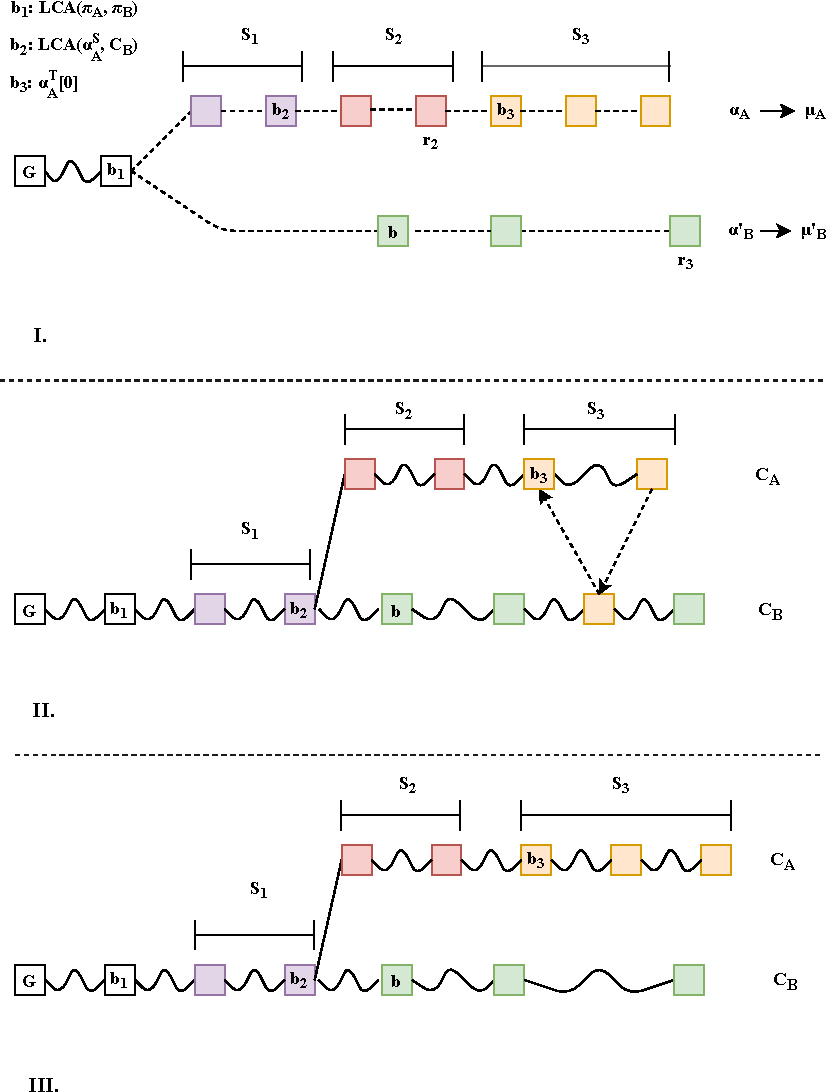
\includegraphics[scale=0.65]{figures/proof_velvet-crop.pdf}
	\end{center}
	\caption{\textit{ Wavy lines imply one or more blocks. Dashed lines and arrows imply interlink pointers to superblocks. \textbf{I}: the three round sets in two competing proofs at different levels, \textbf{II}: the corresponding 0-level blocks implied by the two proofs, \textbf{III}: blocks participating in chain $\chain_B$ and block set $\widetilde{\chain}_\mathcal{A}$ from the verifier's perspective.}}
    \label{fig:proof_velvet}
\end{figure}

We will now show three successive claims under velvet fork conditions: First that $\alpha_\mathcal{A}^1$ contains only a few blocks. Second,  $\alpha_\mathcal{A}^2$ contains only a few blocks. And third, the adversary is able to produce a winning $a_\mathcal{A}$ with negligible probability.\\

\textbf{Claim 1:} $\alpha_\mathcal{A}^1 = \alpha_\mathcal{A}(b_0 : b_1]$ contains only a few blocks. We have defined $b_0 = LCA(\pi_\mathcal{A}, \pi_B)$ and $b_1 = LCA(\alpha^{\mathcal{S}}_\mathcal{A}, \alpha'_B \downarrow)$. First observe that there are no thorny blocks in $\alpha_\mathcal{A}^1$ since $\alpha_\mathcal{A}^1[-1] = b_1$ is a smooth block. This means that if $b_1$ was generated at round $r_{b_1}$ and $\alpha^{\mathcal{S}}_\mathcal{A}[-1]$ in round $r$, then $r \geq r_{b_1}$. So, $\alpha_\mathcal{A}^1$ consists a valid chain. We show the statement considering the two possible cases for the relation of $\mu_\mathcal{A}, \mu'_B$.

\textit{\underline{Claim 1a}:} If $\mu'_B \leq \mu_A$ then they are completely disjoint. In such a case of inequality, every block in $\alpha_A$ would also be of lower level $\mu'_B$. Because of the adequate level $\mu'_B$ we know that $C\{b{:}\}\upchain^{\mu'_B} = \pi\{b{:}\}\upchain^{\mu'_B}$\cite{nipopows}. Subsequently, any block in $\pi_A\upchain^{\mu_A}\{b{:}\}[1{:}]$ would also be included in proof $\alpha'_B$, but $b=LCA(\pi_A, \pi_B)$ so there can be no succeeding block common in $\alpha_A, \alpha'_B$.

\textit{\underline{Claim 1b}:} If  $\mu'_B > \mu_A$ then $\lvert \alpha_A[1{:}]  \cap \alpha'_B\downarrow[1{:}] \rvert = k_1 \leq g(2^{\mu'_B - \mu_A})$.\\
Let's call $b$ the first block in $\alpha'_B$ after block $b_0$. Suppose for contradiction that $k_1 > g(2^{\mu'_B - \mu_A})$.  Since block $b$ of level $\mu'_B$ is also of level $\mu_A$, the adversary could include it in the proof but $b$ cannot exist in both $\alpha_A, \alpha'_B$ since $\alpha_A \cap \alpha'_B = \emptyset$ by definition. In case that the adversary chooses not to include $b$ in the proof then she can include no other blocks of $\chain_B$ in her proof, since it would not consist a valid chain. Therefore, the adversary can include at most the $\mu_\mathcal{A}$ upgraded  blocks  between  $b_0$, $b$, which are expected to be equal to $g(2^{\mu'_B - \mu_A})$.

We conclude that $\lvert \alpha^{\mathcal{S}}_\mathcal{A} \cap \alpha'_B\downarrow[1{:}] \rvert = k_{1} \leq g(2^{\mu'_B - \mu_\mathcal{A}}) $, where $g$ the velvet parameter denoting the percentage of upgraded honest parties.

Consequently, there are at least $\lvert\alpha_\mathcal{A}\rvert - k_1$ blocks after block $b$ in $\alpha_\mathcal{A}$ which are not honestly generated blocks existing in $\chain_B$. In other words, there are $\vert \alpha_\mathcal{A} \vert - k_1$ blocks after block $b$ in $\alpha_\mathcal{A}$, which are either thorny blocks existing in $\chain_B$ either don't belong in $\chain_B$.\\

\textbf{Claim 2.}
Part $\alpha_\mathcal{A}^2 = \alpha_\mathcal{A}(b_1:b_2]$ consists of only a few blocks. Let $ \lvert \alpha_\mathcal{A}^2 \rvert = k_2$. We have defined $b_2 = \alpha_\mathcal{A}^2[-1]$ to be the last block generated by an honest player in $\alpha_\mathcal{A}$. Consequently no thorny block exists in $\alpha_\mathcal{A}^2$, so all blocks in this part belong in a proper zero-level chain $\chain_\mathcal{A}^2$.  Let $r_{b_1}$ be the round at which $b_1$ was generated. Since $b_1$ is the last block in $\alpha_\mathcal{A}$ which belongs in $\chain_B$, then $\chain_\mathcal{A}^2$ is a fork chain to $\chain_B$ at some block $b'$ generated at round $r' \geq r_{b_1}$.

Let $r_2$ be the round when $b_2$ was generated by an honest party. Because an honest party has chain $\chain_B$ at later round $r_3$ when the proof $\pi_B$ is constructed and because of the Common Prefix property on parameter $k_{2\downarrow} = g \cdot 2^{\mu_\mathcal{A}} \cdot k_2$, we conclude that $k_2 \leq k$.

\textbf{Claim 3.} The adversary may submit a suffix proof such that $\lvert \alpha_\mathcal{A}\rvert \geq \lvert \alpha_B \rvert$ with negligible probability. As explained earlier part $\alpha^3_\mathcal{A}$ consists only of adversarially generated blocks. The security parameter $m$ guarantees that $\lvert \alpha^3_\mathcal{A} \rvert > k$, as will be later presented in detail. Let $U$ be the set of consecutive rounds $r_2...r_3$. Then all $k_3$ blocks of this part of the proof are generated during $U$. Let $\alpha'^{S_3}_B$ be the last part of the honest proof containing the interlinked $\mu_B$ superblocks generated during $U$. Then from lemma \ref{lem:claim3_lemma} we have that $ 2^{\mu_\mathcal{A}}\lvert \alpha^3_\mathcal{A} \rvert < 2^{\mu_B} \lvert \alpha'^U_{B}\upchain^{\mu_B} \rvert $.

From all the above Claims we have that:\\
For the first round set $S_1$, because of the common underlying chain:
\begin{equation} \label{eq_v_round_set_1}
2^{\mu_\mathcal{A}} \lvert \alpha_\mathcal{A}^{S_1} \rvert \leq 2^{\mu'_B} \lvert \alpha'{_B^{S_1}} \rvert
\end{equation}
For the second round set $S_2$ because of the adoption by an honest party of chain $\chain_B$ at a later round $r_3$ we have:
\begin{equation} \label{eq_v_round_set_2}
	2^{\mu_\mathcal{A}} \lvert \alpha_\mathcal{A}^{S_2} \rvert \leq 2^{\mu'_B} \lvert \alpha'{_B^{S_2}} \rvert
\end{equation}
For the third round set $S_3$ we have:
\begin{equation} \label{eq_v_round_set_3}
	2^{\mu_\mathcal{A}} \lvert \alpha_\mathcal{A}^{S_3} \rvert < 2^{\mu'_B} \lvert \alpha'{_B^{S_3}} \rvert
\end{equation}
Consequently we have:

\begin{equation*}
	2^{\mu_\mathcal{A}} ( \vert \alpha_\mathcal{A}^{S_1} \vert + \vert \alpha_\mathcal{A}^{S_2} \vert + \vert \alpha_\mathcal{A}^{S_3} \vert ) < 2^{\mu'_B} ( \vert \alpha'{_B^{S_1}} \vert + \vert \alpha'{_B^{S_2}} \vert + \vert \alpha'{_B^{S_3}} \vert) \Rightarrow
\end{equation*}

\begin{equation} \label{eq_v_all_round_sets}
	2^{\mu_\mathcal{A}} \vert \alpha_\mathcal{A} \vert < 2^{\mu'_B} \vert \alpha'{_B} \vert
\end{equation}

Therefore we have proven that $2^{\mu'_B} \vert \pi_B \upchain^{\mu'_B} \vert > 2^{\mu_\mathcal{A}} \vert \pi_\mathcal{A}^{\mu_\mathcal{A}} \vert$. From the definition of $\mu_B$, we know that $2^{\mu_B} \vert \pi_B \upchain^{\mu_B} \vert > 2^{\mu'_B} \vert \pi_B \upchain^{\mu'_B} \vert$ because it was chosen $\mu_B$ as level of comparison by the Verifier. So we conclude that $2^{\mu_B} \vert \pi_B \upchain^{\mu_B} \vert > 2^{\mu_\mathcal{A}} \vert \pi_\mathcal{A} \upchain^{\mu_\mathcal{A}} \vert$.
\end{proof}
